\chapter{Terrain Classification for AMOS II} \label{chapter:05:terrain_classification}
Classification, one of the most widely used areas of machine learning, has a broad array of applications (see \cref{chapter:01:introduction}). To fit a classifier to a problem, one needs to define a problem data structure. Data consists of samples and discrete targets, often called classes. The samples are sooner or later converted into so called feature vectors of a fixed length. The lenght of feature vectors usually determines an input of chosen classifier and number of classes sets an output.

The classification problem in this thesis relates to AMOS II, an open-source multi sensori-motor robotic platform (see \cref{img:amosii}). The task is to classify various terrain types, while the only input comes from proprioceptive sensors. The overall process is based on simulation data and as \cref{chapter:04:neural_net_implementation} reveals, feedforward neural networks are involved.

\section{Overall Process Summary} \label{sec:overall_process_summary}
The very first step is to make the AMOS II simulation run (\cref{ssec:lpzrobots_sim}). Then a simple tripod gait controller is implemented (\cref{ssec:tripod_gait_controller}). To generate various terrain types, the number of variable terrain quailities and their ranges are determined (\cref{ssec:terrain_qualities}). Based on these qualities (parameters), a number of virtual terrains is defined (\cref{ssec:terrain_parameters}) and an optimality of these parameters is briefly analysed (\cref{ssec:terrains_analysis}).

Next, AMOS II (its simulation alternative) is forced to walk on every defined terrain type several times and for a sufficiently long period of time and data from all proprioceptors are saved. This data is then verified and failing experiments are removed. The data acquisition step is parameterized by a standard deviation of additive (Guassian) terrain noise and is run for several values.

Having a clean simulation data from all sensors, a feature vector structure is determined. Then a Gaussian signal noise is added. Finally, a dataset is created by splitting all the data into training, validation and testing sets. As it is indicated on \cref{img:terrain_classification_process}, several datesets and several classifiers are generated during the process. 

An optimal neural network classifier is found. The optimal network is then pruned by the algorithm developed in section X. Classification performance of developed tools are compared to a \textit{Scikit-learn} network classification library sknn [].

\begin{figure}[H]
  \centering
  \includegraphics[width=1.0\textwidth]{terrain_classification_process}
  \caption{Terrain classification process - overall diagram.}
  \label{img:terrain_classification_process}
\end{figure}

The dataset packages may differ in these parameters:
\begin{itemize}
\item terrain types included (-> number of classes)
\item sensors on input
\item samples length (number of simulation timesteps)
\item terrain noise and signal noise
\item number of samples
\end{itemize}

The trained networks may differ in following parameters:
\begin{itemize}
\item neural network structure
\item accuracy on training/validation/testing sets 
\end{itemize}

\section{Experimental Environment Specification}
Naturally, the idea of the research is to implement an online terrain classifier on the real machine. Therefore the target robot is described in the following section (\ref{ssec:amosii}).

Nevertheless, it is usually a good idea to base the reasearch on simulation data if a satisfactory simulator is available. In this case, \textit{LPZ Robots} \citep{misc:lpzrobots} is used (\cref{ssec:lpzrobots_sim}).

\subsection{Hexapod Robot AMOS II} \label{ssec:amosii}
The \textit{AMOS II} abbreviation stands for Advanced Mobility Sensor Driven-Walking Device - version II. It is a biologically inspired hardware platform of size 30x40x20 cm and weight 5.8 Kg (see \cref{img:amosii}). It is mainly used to perform experiments with neural control, memory and learning on a device with many degrees of freedom and to study the coordination of it \citep{misc:amosii}.

\begin{figure}[H]
  \centering
  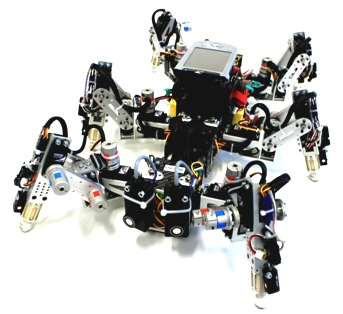
\includegraphics[width=343px]{amosii}
  \caption{AMOS II. \citep{misc:amosii}}
  \label{img:amosii}
\end{figure}

In general, the robot serves as a hardware platform for neural perception-action systems experiments. The body parts are modeled on the basis of robot's biological inspiration - a cockroach.

A wide range of sensors allows AMOS II to perform several autonomous behaviours. However, only the proprioceptive sensors are important for this research, therefore, we focus on angle sensors and foot contact sensors. All of them are located on robot's legs, so the leg structure is shown on \cref{img:amosii_leg}.

\begin{figure}[H]
  \centering
  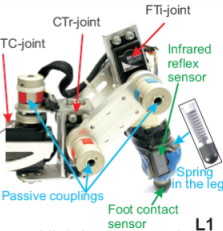
\includegraphics[width=225px]{amosii_leg}
  \caption{AMOS II. \citep{misc:amosii}}
  \label{img:amosii_leg}
\end{figure}

As figures \ref{img:amosii} and \ref{img:amosii_leg} reveal, the robot has \textbf{6 foot contact sensors} in total, one on each leg. Each of them returns a value from range $ [0.0, 1.0] $ depending on how strong the foot contact is - it is equal $ 1.0 $ if the robot stands on the leg with its full weight and it equals $ 0.0 $ when the leg is in the air.

There are three joints on each of robots legs. The thoraco-coxal (TC-) joint is responsible for forward/backward movements. The coxa-trochanteral (CTr-) joint enables elevation and depression of the leg and the last one, femur-tibia (FTi-) joint is used for extension and flexion of the tibia.

These joints are physically actuated by standard servo motors. Having the servos positions, angles of the joints are known and are also considered as propriceptive sensors. As AMOS II has six legs and there are three joints on each leg, there are \textbf{18 angle sensors} in total. There is also one backbone joint angle, however, as this one is not implemented in the simulation (see \cref{ssec:lpzrobots_sim}), it is omitted in this research.

In \cref{tab:proprioceptors} there are all the propriceptors, their shortcuts and original ranges listed. The ranges are based on the individual servos locations and are explicitly set up to avoid collisions. In \cref{sec:feature_vector_building} a normalization of these ranges is discussed.

Regarding robots actuators, the servo motors can produce variably compliant motions as if each of them were driven by a pair of agonist and antagonist muscles (see \cite{misc:amosii} for details). 

\begin{table}[H]
\centering
\caption{AMOS II - Proprioceptive sensors}
\label{tab:proprioceptors}
\begin{tabular}{|l|l|c|}
\hline
\textit{shortcut} & \multicolumn{1}{c|}{\textit{sensor description}} & \textit{original range} \\ \hline
\textbf{ATRf}         & Angle sensor, Thoraco joint, Right front leg     &                         \\ \hline
\textbf{ATRm}         & Angle sensor, Thoraco joint, Right middle leg    &                         \\ \hline
\textbf{ATRh}         & Angle sensor, Thoraco joint, Right hind leg      &                         \\ \hline
\textbf{ATLf}         & Angle sensor, Thoraco joint, Left front leg      &                         \\ \hline
\textbf{ATLm}         & Angle sensor, Thoraco joint, Left middle leg     &                         \\ \hline
\textbf{ATLh}         & Angle sensor, Thoraco joint, Left hind leg       &                         \\ \hline
\textbf{ACRf}         & Angle sensor, Coxa joint, Right front leg        &                         \\ \hline
\textbf{ACRm}         & Angle sensor, Coxa joint, Right middle leg       &                         \\ \hline
\textbf{ACRh}         & Angle sensor, Coxa joint, Right hind leg         &                         \\ \hline
\textbf{ACLf}         & Angle sensor, Coxa joint, Left front leg         &                         \\ \hline
\textbf{ACLm}         & Angle sensor, Coxa joint, Left middle leg        &                         \\ \hline
\textbf{ACLh}         & Angle sensor, Coxa joint, Left hind leg          &                         \\ \hline
\textbf{AFRf}         & Angle sensor, Femur joint, Right front leg       &                         \\ \hline
\textbf{AFRm}         & Angle sensor, Femur joint, Right middle leg      &                         \\ \hline
\textbf{AFRh}         & Angle sensor, Femur joint, Right hind leg        &                         \\ \hline
\textbf{AFLf}         & Angle sensor, Femur joint, Left front leg        &                         \\ \hline
\textbf{AFLm}         & Angle sensor, Femur joint, Left middle leg       &                         \\ \hline
\textbf{AFLh}         & Angle sensor, Femur joint, Left hind leg         &                         \\ \hline
\textbf{FRf}          & Foot contact sensor, Right front leg             & {[}0.0, 1.0{]}          \\ \hline
\textbf{FRm}          & Foot contact sensor, Right middle leg            & {[}0.0,1.0{]}           \\ \hline
\textbf{FRh}          & Foot contact sensor, Right hind leg              & {[}0.0, 1.0{]}          \\ \hline
\textbf{FLf}          & Foot contact sensor, Left front leg              & {[}0.0, 1.0{]}          \\ \hline
\textbf{FLm}          & Foot contact sensor, Left middle leg             & {[}0.0, 1.0{]}          \\ \hline
\textbf{FLh}          & Foot contact sensor, Left hind leg               & {[}0.0, 1.0{]}          \\ \hline
\end{tabular}
\end{table}

For purposes of this thesis, it is enough to know that it is possible to generate various gaits using the joints actuators and robots neural locomotion control. The gait controller used for this research is described in \cref{ssec:tripod_gait_controller}.

\subsection{LPZ Robots Simulation} \label{ssec:lpzrobots_sim}
The \textit{lpzrobots} project, developed by a research group at the University of Leipzig \citep{misc:lpzrobots} under GPL license, contains many subprojects. For purposes of this thesis, the most important ones are:

\begin{description}
\item[selforg] : homeokinetic controllers implementation framework
\item[ode\_robots] : a 3D physically correct robot simulator
\end{description}

The project is implemented in \textit{C++} and needs an Unix system to be run. It consists of two main GIT repositories to be forked - lpzrobots and go\_robots. The overall software architecture is shown on \cref{img:lpzrobots_architecture}.

\begin{figure}[H]
  \centering
  \includegraphics[width=0.5\textwidth]{lpzrobots_architecture}
  \caption{Software architecture for LPZRobots and GoRobots. \citep{misc:lpzrobots}}
  \label{img:lpzrobots_architecture}
\end{figure}

To introduce the elements in \cref{img:lpzrobots_architecture}, \textit{ThisSim} is an inherited class of another class called \textit{Simulation} and is initialized everytime the simulation is launched. It integrates all elements together, controls the environment as well as the robot and sets up initial parameters.

An instance of the \textit{Agent} class integrates all components of the agent (robot) by using the shown classes.

\begin{figure}[H]
  \centering
  \includegraphics[width=1.0\textwidth]{lpzrobots_repos}
  \caption{Structure of the two repositories (LPZRobots and GoRobots). \citep{misc:lpzrobots}}
  \label{img:lpzrobots_repos}
\end{figure}

On \cref{img:lpzrobots_repos} the cooperation of the two repositories is illustrated. With reference to \cref{app:code_documentation}, one can call the \textit{main.cpp} file from \textit{root/simulation/mbulinai22015-gorobots\_edu-fork/practices/amosii} directory as the main simulation file for purposes of the thesis. It sets up the environment with initial parameters $ controlinterval = 10 $ and $ simstepsize = 0.01 $, which means the simulation sensitivity is \textit{10 steps} per second.

It also sets the initial camera and robot position in the map. The robot position is chosen randomly and the reason for that is described in \cref{sec:data_acquisition}. The robot fixator, which is originally implemented for AMOS II is removed, so the robot starts walking right after the simulation is launched.

The \textit{main.cpp} file contains all terrain types parameters introduced in \cref{sec:virtual_terrain_types}. The required terrain to be simulated is then passed to this file as an argument. Additionally, the standard deviation value of Gaussian terrain noise (details in \cref{ssec:terrain_noise}) is set as another argument. Finally, the file is ready to take one more argument, which is a simulation noise represented by a float number. In this research it is fixed to zero though and only the terrain noise combined with a signal noise are used.

The virtual vizualization of AMOS II is illustrated on \cref{img:amosii_sim}.

\begin{figure}[H]
  \centering
  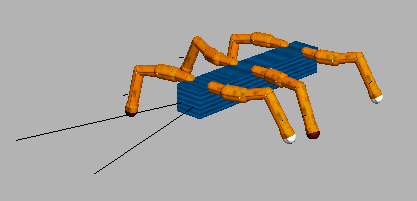
\includegraphics[width=0.8\textwidth]{amosii_sim}
  \caption{Simulation alternative for AMOS II.}
  \label{img:amosii_sim}
\end{figure}

\subsection{Tripod Gait Controller} \label{ssec:tripod_gait_controller}
The main motivation for terrain classification is to adjust current robot's gait accordingly and save some energy thereby. It is assumed that the robot is already walking, using some implemented gait, when it tries to classify the terrain. Hence, it is needed to make the simulation agent walk as well. The starting gait is decided to be the \textbf{tripod} gait.

To generate a tripod gate, a central pattern generator (CPG) is used. \citep{unpub:ai3_lec3} It is implemented as a 2-neuron neural network right inside AMOS II (\cref{img:two_neuron_network}).

\begin{figure}[H]
  \centering
  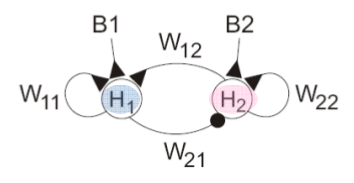
\includegraphics[width=0.5\textwidth]{two_neuron_network}
  \caption{2-neuron network oscillator. \citep{unpub:ai3_lec3}}
  \label{img:two_neuron_network}
\end{figure}

To make it work in practise, \textit{tripod\_controller.h} is written. Its initial conditions and parameters are shown in \cref{code:tripod_init}.

\begin{lstlisting}[language=C++, caption={Initialization in tripod\_controller.h}, label=code:tripod_init]
aH1 = 0; aH2 = 0;            // activities
bH1 = 0; bH2 = 0;            // biases
oH1 = 0.001; oH2 = 0.001;    // outputs
wH1H1 = 1.4; wH1H2 = 0.4;    // weights to H1
wH2H2 = 1.4; wH2H1 = -0.4;   // weights to H2
p1 = 0.35;                   // parameter for Thoraco joints
p2 = 0.3;                    // parameter for Coxa joints
\end{lstlisting}

Then, during the simulation, in \textit{tripod\_controller.h} there is a function called \textit{step()} able to control robots joints in every single simulation step. In this function three important actions come about.

\begin{enumerate}
\item \textbf{The activation function}
\begin{equation}
a_i(t+1) = \displaystyle\sum_{j=1}^{n} w_{ij}o_j(t) + b_i, i = 1, ..., n
\end{equation}

In this case, the following happens:
\begin{equation}
\begin{split}
a_{H_1} = w_{H_1,H_1} * o_{H_1} + w_{H_1,H_2} * o_{H_2} + b_{H_1} \\
a_{H_2} = w_{H_2,H_2} * o_{H_2} + w_{H_2,H_1} * o_{H_1} + b_{H_2}
\end{split}
\end{equation}

\item \textbf{The transfer function}
\begin{equation}
f(a_i) = tanh(a_i) = \frac{2}{1+e^{-2a_i}} - 1
\end{equation}

\begin{equation}
\begin{split}
o_{H_1} = tanh(a_{H_1}) \\
o_{H_2} = tanh(a_{H_2})
\end{split}
\end{equation}

\item \textbf{Joints settings}
With the reference to previous equations and variables names, the actuators are set in the sense shown on \cref{img:tripod_illustration}. The \textit{femur} joints (red ones) stay unchanged (set to zero). This settings generates a reliable tripod gait for AMOS II.

\begin{figure}[H]
  \centering
  \includegraphics[width=250px]{tripod_illustration}
  \caption{Tripod gait controller illustration.}
  \label{img:tripod_illustration}
\end{figure}
\end{enumerate}

\section{Virtual Terrain Types} \label{sec:virtual_terrain_types}
Since the verification is based on the simulation only, the goal is to design an authentical virtual environment. For this purpose various terrain types need to be virtually imitated.

Luckily, the \textbf{LpzRobots} AMOS II simulator supports some terrain settings. In the main simulation file (\textit{main.cpp} - see \ref{app:code_documentation}), a \textit{'rough terrain'} substance is being initialized and passed through a handle to a \textit{TerrainGround} constructor.

\begin{lstlisting}[language=C++, caption={Setting a terrain ground in main.cpp}, label=code:terrain_ground]
Substance roughterrainSubstance(terrain_roughness, terrain_slip,
                       terrain_hardness, terrain_elasticity);
oodeHandle.substance = roughterrainSubstance;
TerrainGround* terrainground = new TerrainGround(oodeHandle, 
                       osgHandle.changeColor(terrain_color),
                       "rough1.ppm", "", 20, 25, terrain_height);
\end{lstlisting}

As \cref{code:terrain_ground} shows, the terrain substance is defined by four parameters: \textbf{roughness}, \textbf{slipperiness}, \textbf{hardness} and \textbf{elasticity}.

Besides the substance handle, the \textit{TerrainGround} constructor takes six more arguments.

\begin{description}
\item[terrain\_color] : simulation ground color
\item["rough1.ppm"] : an image in the .ppm format, a lowest common denominator color image file format \citep{misc:ppm}, a bitmap height file
\item[""] : texture image (not used)
\item[20] : walking area x-size 
\item[25] : walking area y-size
\item[terrain\_height] : maximum terrain height
\end{description}

\subsection{Terrain Qualities} \label{ssec:terrain_qualities}
Out of the listed ground parameters, some of them are picked up and being called \textit{terrain qualities}, as they define a specific terrain type.

It has been decided not to change the \textit{.ppm} image for various terrains and so \textit{rough1.ppm} is fixed. Also the walking area is set to (big enough) final size of \textit{20x25}. The color is variable, however, besides the simulation graphics it does not have any effect on results. 

Therefore, a virtual terrain type is defined by five qualitites. Each of them is a float number from an empirically stated range \footnote{The upper range limits have been set up based on significant changes in robot behaviour for various parameter values.}. (\cref{tab:terrain_qualities}).

\begin{table}[H]
\centering
\caption{Terrain qualities and their ranges}
\label{tab:terrain_qualities}
\begin{tabular}{lccll}
             & min value & max value \\
roughness    & 0.0       & 10.0      \\
slipperiness & 0.0       & 100.0     \\
hardness     & 0.0       & 100.0     \\
elasticity   & 0.0       & 2.0       \\
height       & 0.0       & 0.1 
\end{tabular}
\end{table}

\subsection{Terrains Parameters Determination} \label{ssec:terrain_parameters}
To determine a terrain type, one has to come up with the five parameters from \cref{tab:terrain_qualities}.

First, number of identifiable virtual terrain types needs to be determined. For purposes of this thesis, it has been decided to create \textbf{14 terrain types}. Their parameters (showed in \cref{tab:terrains_parameters}) have been set up intuitively, based on the AMOS II simulated behaviour. With respect to the qualities ranges from \cref{tab:terrain_qualities}, the values have been normed to (0, 1).

\begin{table}[H]
\centering
\caption{Virtual terrain types parameters.}
\label{tab:terrains_parameters}
\begin{tabular}{|l|l|c|c|c|c|c|}
\hline
\textit{\#}                                       & \textit{terrain title} & \multicolumn{1}{l|}{\textit{roughness}} & \multicolumn{1}{l|}{\textit{slipperiness}} & \multicolumn{1}{l|}{\textit{hardness}} & \multicolumn{1}{l|}{\textit{elasticity}} & \multicolumn{1}{l|}{\textit{height}} \\ \hline
\cellcolor[HTML]{876496}1                         & \textbf{carpet}        & 0.3                                     & 0.0                                        & 0.4                                    & 0.15                                     & 0.2                                  \\ \hline
\cellcolor[HTML]{9C9FA6}2                         & \textbf{concrete}      & 1.0                                     & 0.0                                        & 1.0                                    & 0.0                                      & 0.0                                  \\ \hline
\cellcolor[HTML]{DCE696}3                         & \textbf{foam}          & 0.5                                     & 0.0                                        & 0.0                                    & 1.0                                      & 0.7                                  \\ \hline
\cellcolor[HTML]{239614}4                         & \textbf{grass}         & 0.5                                     & 0.0                                        & 0.3                                    & 0.3                                      & 0.5                                  \\ \hline
\cellcolor[HTML]{737F9C}5                         & \textbf{gravel}        & 0.7                                     & 0.001                                      & 1.0                                    & 0.0                                      & 0.3                                  \\ \hline
\cellcolor[HTML]{D7E3FF}6                         & \textbf{ice}           & 0.0                                     & 1.0                                        & 1.0                                    & 0.0                                      & 0.0                                  \\ \hline
\cellcolor[HTML]{646464}7                         & \textbf{mud}           & 0.05                                    & 0.05                                       & 0.005                                  & 0.25                                     & 0.2                                  \\ \hline
\cellcolor[HTML]{96FABE}8                         & \textbf{plastic}       & 0.1                                     & 0.02                                       & 0.6                                    & 0.5                                      & 0.0                                  \\ \hline
\cellcolor[HTML]{6E5A3C}9                         & \textbf{rock}          & 1.0                                     & 0.0                                        & 1.0                                    & 0.0                                      & 1.0                                  \\ \hline
\cellcolor[HTML]{000000}{\color[HTML]{FFFFFF} 10} & \textbf{rubber}        & 0.8                                     & 0.0                                        & 0.8                                    & 1.0                                      & 0.0                                  \\ \hline
\cellcolor[HTML]{F2EE7C}11                        & \textbf{sand}          & 0.1                                     & 0.001                                      & 0.3                                    & 0.0                                      & 0.2                                  \\ \hline
\cellcolor[HTML]{FDB0FB}12                        & \textbf{snow}          & 0.0                                     & 0.8                                        & 0.2                                    & 0.0                                      & 0.2                                  \\ \hline
\cellcolor[HTML]{324B32}13                        & \textbf{swamp}         & 0.0                                     & 0.05                                       & 0.0                                    & 0.0                                      & 1.0                                  \\ \hline
\cellcolor[HTML]{5A4100}14                        & \textbf{wood}          & 0.6                                     & 0.0                                        & 0.8                                    & 0.1                                      & 0.2                                  \\ \hline
\end{tabular}
\end{table}

Colors linked to the terrains in \cref{tab:terrains_parameters} are used in the simulation as well as in the figures in Results section.

\subsection{Analysis of Chosen Parameters} \label{ssec:terrains_analysis}
In general, proper data preparation is an important part of classification tasks, hence a brief analysis is presented.

The goal is to imitate real terrains authentically as possible and at the same time to generate such terrains, that are clearly distinguishable from each other. The more two terrains differ the better classification results are expected.

Having five terrain qualities calls for a 5-D space, which is difficult to illustrate or even imagine. Therefore, formula \ref{eq:similarity_factor} is used to compute a similarity factor of two terrain types (the five qualities are listed in \cref{tab:terrain_qualities} and \cref{tab:terrains_parameters}).


\begin{equation} 
\label{eq:similarity_factor}
  SF_{t_1, t_2} = \displaystyle\sum_{i=1}^{5} \abs{quality(i, t_1) - quality(i, t_2)}
\end{equation} 

Naturally, equation \ref{eq:similarity_factor} ends up with $ SF_{similar} = 0.0 $ for two terrains with exactly same parameters and $ SF_{different} = 5.0 $ for two terrains differing most possibly.

The following figure (\ref{fig:terrains_parameters}) shows the variability (similarity factors) of generated terrains.

\begin{figure}[H]
  \centering
  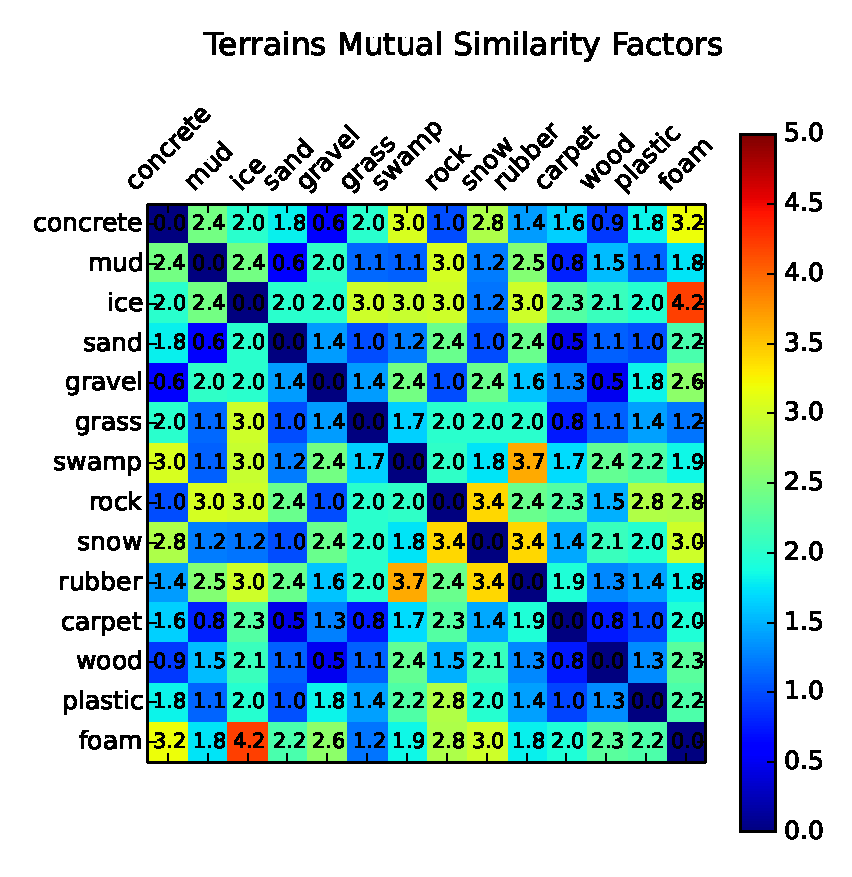
\includegraphics[width=1.0\textwidth]{terrains_variability.eps}
  \caption{Variability of generated terrain types.}
  \label{fig:terrains_parameters}
\end{figure}

Based on \cref{fig:terrains_parameters}, one can say that foam is very different to ice or, for instance, sand is quite similar to mud. The surfaces are virtually generated and their authenticity has not been verified. 

\subsection{Terrain Noise} \label{ssec:terrain_noise}
Generally, using simulation data for the very first research steps brings many benefits and it is usually the right way to start. However, the real world is always different to the simulated alternative and these disparities may influence the results significantly.

In this case, there are some virtually created terrain types based on five qualities (\cref{ssec:terrain_qualities}). These parameters have been set up basically by a guess, intuitively. Therefore, one should assume that the real terrains might be distinct from the virtual ones in some way.

Secondly, if there is a terrain defined as grass for instance, this definition can not be general on no account. There are many different types of grass and they differ from each other at least in the reffered qualities.

Consequently, there are some lines of code added to \textit{main.cpp} (see \ref{app:code_documentation}) enabling to noise the parameters shown in \cref{tab:terrains_parameters}. The following box (\ref{code:terrain_noise}) shows how it is done. 

\begin{lstlisting}[language=C++, caption={Adding terrain noise in main.cpp}, label=code:terrain_noise]
terrain_roughness += fRand(-10.0*std_vol, 10.0*std_vol);
terrain_slip  += fRand(-10.0*std_vol, 10.0*std_vol);
terrain_hardness += fRand(-100.0*std_vol, 100.0*std_vol);
terrain_elasticity += fRand(-2.0*std_vol, 2.0*std_vol);
terrain_height += fRand(-0.1*std_vol, 0.1*std_vol);
    
// limits : params can not be negative
terrain_roughness = max(0.0, terrain_roughness);
terrain_slip = max(0.0, terrain_slip);
terrain_hardness = max(0.0, terrain_hardness);
terrain_elasticity = max(0.0, terrain_elasticity);
terrain_height = max(0.0, terrain_height);
\end{lstlisting}

The \textit{std\_vol} variable comes as an argument to \textit{main.cpp}. It is meant to be a standard deviation of Gaussian noise in percentage. Hence, this percentage is then multiplied with the corresponding quality range and passed to the \textit{fRand()} function in order to generate a random float number from the created range with zero mean.

The function generating the random number uses the \textit{normal (Gaussian) distribution} with a probability density function defined as:

\begin{equation} \label{eq:gaussian_distribution}
p(z) = \frac{1}{\sigma \sqrt{2 \pi}} e^{- \frac{(z-\mu)^2}{2 \sigma^2}}
\end{equation}

In this case the mean $ \mu = 0 $ and the standard deviation $ \sigma $ is defined by a corresponding range percentage. As the values at any pair of times are identically distributed and statistically independent (and hence uncorrelated) \citep{misc:wiki}, a \textbf{white Gaussian noise} is being generated thereby. Additionally, there is some limits checking as the parameters can not take negative values.

In this manner, the terrain types parameters from \cref{tab:terrains_parameters} can be noised, where the magnitude of noise influence is passed as a simulation argument.

\section{Data Acquisition} \label{sec:data_acquisition}
At this point the simulation is set up and ready to be launched. There are \textbf{14} virtually created terrain types (defined in \cref{sec:virtual_terrain_types}, \cref{tab:terrains_parameters}) and \textbf{24} robot's proprioceptive sensors (described in \cref{ssec:amosii}, \cref{tab:proprioceptors}) available.

Predictably, the terrain types are assumed to be classification targets (classes). Therefore, some data needs to be generated for each of these classes. This data comes from the 24 proprioceptors and one needs to find a way how to form feature vectors (classification samples) out of it (\cref{sec:feature_vector_building}), which is one of the most essential parts of the process.

As it is later described in more detail, several sensors values in time need to be used to catch the robot's dynamics on various terrains. Therefore, to generate a single data example, the simulation must be run for a period of time. The optimal duration is not known yet, but besides this fact, one should start thinking how to generate a sufficient amount of samples for classification at this point.

The very simple way might be to let the robot walk for a long period of time and then just to cut the signals coming from sensors into many samples, based on an estimated timestep. The hitch of this approach is in initial conditions - they would become the same for every sample, which is not correct.

To keep the rightness, the simulator is launched several times in order to generate several samples for every terrain type. It has been decided to let the robot walk for \textbf{10} seconds each time. In combination with the simulation settings (see \cref{ssec:lpzrobots_sim}), this implies \textbf{100} values for every sensor and for every simulation run - which should be more than enough.

For illustration, data from sensor \textit{ATRf} acquired when the robot was walking on a \textit{concrete} surface for approximately 10 seconds is shown on \cref{fig:data_example}.

\begin{figure}[H]
  \centering
  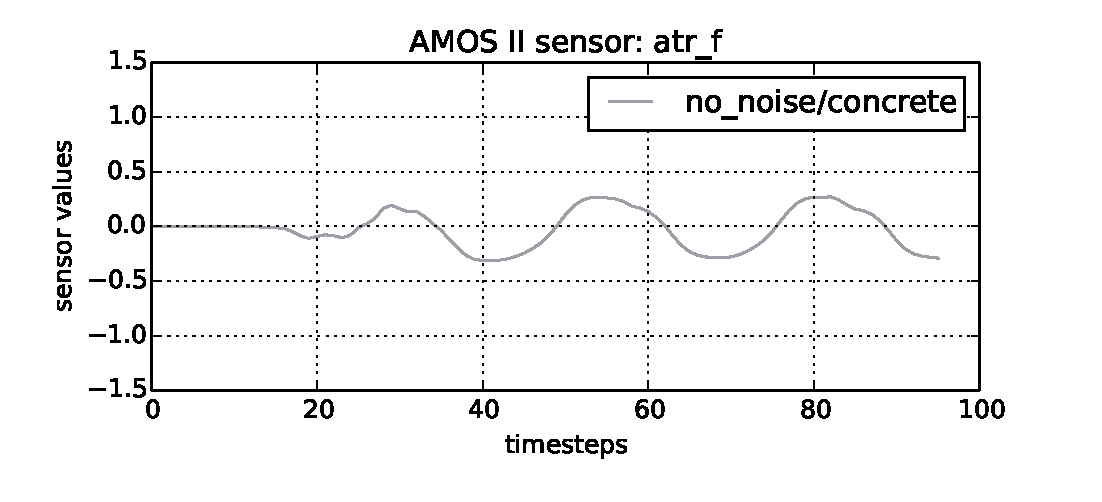
\includegraphics[width=1.0\textwidth]{plot_sensor_atr_f_nn_concrete.eps}
  \caption{Data example: ATRf, concrete, 10 seconds}
  \label{fig:data_example}
\end{figure}

The \textit{no\_noise} indication in the figure legend reffers to \cref{ssec:terrain_noise}. An optimal starndard deviation value of the additive Gaussian noise is not known. Therefore data for several values of this parameter has been generated. The simulation has been gradually run for:

\begin{itemize}
\item $ \sigma_p = 0.0 $ (no noise)
\item $ \sigma_p = 0.01 $ (noise 1\%)
\item $ \sigma_p = 0.03 $ (noise 3\%)
\item $ \sigma_p = 0.05 $ (noise 5\%)
\item $ \sigma_p = 0.1 $ (noise 10\%)
\item $ \sigma_p = 0.2 $ (noise 20\%)
\end{itemize}

The $ \sigma_p $ is a standard deviation percentage, as shown in \cref{code:terrain_noise}, this $ \sigma_p $ is applied on qualities ranges and so corresponding standard deviation values $ \sigma_i $ are computed.

It is always recommended to store rough data before some processing, hence the simulator creates \textit{.txt} files of structure symbolized in \cref{txt:rough_data} (with the reference to sensors shortcuts in \cref{tab:proprioceptors}). 

\begin{lstlisting}[language=XML, caption={Rough sensory data files structure}, label=txt:rough_data]
timestep_001;ATRf;ATRm;ATRh;ATLf;...;FRh;FLf;FLm;FLh
timestep_002;ATRf;ATRm;ATRh;ATLf;...;FRh;FLf;FLm;FLh
...
timestep_100;ATRf;ATRm;ATRh;ATLf;...;FRh;FLf;FLm;FLh
\end{lstlisting}

There is a \textit{.txt} file of this structure for every single simulation run in the \textit{root/data/} directory (see \cref{app:code_documentation}).

All the data files are generated by a script called \textit{generate\_txt\_data.py} (\ref{app:code_documentation}). This script takes several arguments, like number of jobs (simulation runs), terrain types involved or the terrain noise \textit{std} ($ \sigma_p $). Then a loop based on these parameters starts, where the simulation is launched and stopped after ten seconds each iteration. This is performed by calling a bash command (since the simulation is \textit{.cpp} based) and then killing the called process from python. The corresponding \textit{.txt} file is saved after each iteration by the simulation and then copied by the python script to a corresponding folder in \textit{root/data/}.

\begin{figure}[H]
  \centering
  \includegraphics[width=0.8\textwidth]{generating_data}
  \caption{The process of data acquisition from the simulation.}
  \label{img:generating_data}
\end{figure}

In this manner, \textit{.txt} files for all terrains and all mentioned $ \sigma_p $ are saved into a structure illustrated on \cref{img:data_dir_structure}. Each \textit{.txt} file contains approximately 100 lines, one for each simulation step (as shown in \cref{txt:rough_data}). Every line then contains values of the 24 proprioceptive sensors.

\begin{figure}[H]
  \centering
  \includegraphics[width=0.8\textwidth]{data_dir_structure}
  \caption{The structure of rough data directory.}
  \label{img:data_dir_structure}
\end{figure}

Right after the data generation, a script called \textit{clean\_txt\_data.py} (\ref{app:code_documentation}) is used to check the created \textit{.txt} files. As it takes a long time to generate all the data, sometimes the simulation fails and the files are incomplete. Hence the script checks whether there are enough timesteps (at least more than 95) and also if the steps are not messed. Files that fail during the inspection are removed.
to create
As \cref{img:data_dir_structure} reveals, there are \textbf{500} \textit{.txt} files for every \textit{noise/terrain} configuration. This allows creating datasets of 500 samples per class.

\section{Feature Vector Compilation} \label{sec:feature_vector_compilation}
So far, the hexapod simulation has been introduced, virtual terrain types defined and the simulator has been run on these terrains and for various values of terrain noise power. All the data has been acquired from the simulation as \textit{.txt} files. Hence the simulation is not needed anymore and only the gathered data are used for the following processing.

Classification tasks are generally based on datasets consisting of samples and corresponding targets. The samples need to be represented in a numerical way in order to be processed by a computer and its appropriate algorithms. In machine learning, this numerical representation of an object is called \textit{a feature vector}, an n-dimensional vector of numerical values. This section is devoted to building a feature vector out of the data gathered from proprioceptive sensors.

This part of the process is crucial as the way of feature vector compilation can influence classification results a lot. Information loss or redundant structures are quite frequent mistakes here. Therefore, as the optimal structure is not known, several possibilities are tested again and therefore some new process parameters appear at this point (mentioned already in \cref{sec:overall_process_summary}).

For this particular problem, the task is to form a feature vector out of content of one \textit{.txt} file (got in \cref{sec:data_acquisition}), as each of these files contains data for one sample (see \cref{img:feature_vector_forming}).

\begin{figure}[H]
  \centering
  \includegraphics[width=1.0\textwidth]{feature_vector_forming}
  \caption{Forming a feature vector out of a data file.}
  \label{img:feature_vector_forming}
\end{figure}

At this point, one may ask for the reason of using several timesteps for creating one sample. It is assumed that a proper terrain classification using proprioceptors at one moment in time is at least difficult, if not impossible. Therefore the idea is to let the robot walk for a while and take down the dynamics of the sensors. Of course, the more timesteps are used for one sample, the more time the classification takes. Because of these arguments the number of timesteps is left as a global process parameter and it is a subject for later discussion.

Sensors to be used is another global parameter coming out of this section. The anticipation is that the feature vector becomes redundant using all of the 24 sensors, as many of them might behave similarly. However, for now all of them are used to show how the feature vector is built and it is also left for later discussion.

Parameters for discussion coming out of feature vector compilation:
\begin{itemize}
\item number of timesteps used to build one feature vector (one sample)
\item sensors involved in classification
\end{itemize}

Now, with reference to \cref{img:feature_vector_forming}, the question is how to transform the \textbf{2D} data from \textit{.txt} files into \textbf{1D} vectors. The idea is to fix the \textit{timesteps} parameter and arrange the columns of the matrix into one vector. This implies having data from all sensors one by one next to each other and forming one feature vector together. 

On \cref{fig:sample_example} an example of this kind of forming is shown. For illustration there is just one terrain type (\textit{concrete}) involved. The number of timesteps is set to 10 and all 24 sensors are used, hence a feature vector of length 240 is gained. The corresponding sensors shortcuts (see \cref{tab:proprioceptors}) are added to the x-axis annotation. The 18 angle sensors are followed by the 6 foot contact sensors.

\begin{figure}[H]
  \centering
  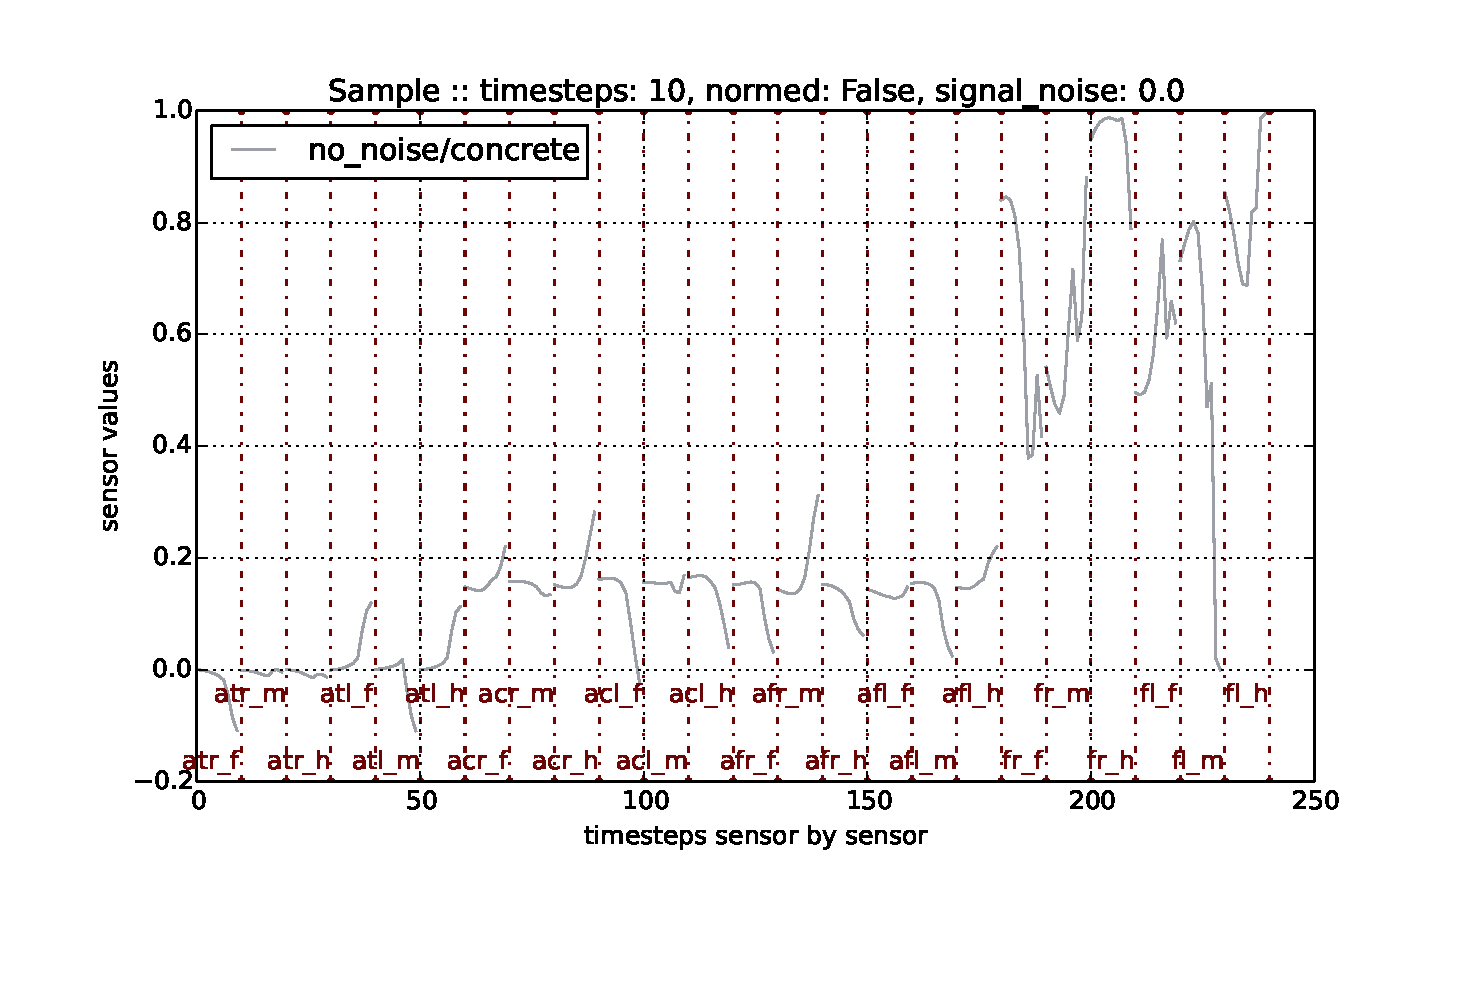
\includegraphics[width=1.0\textwidth]{sample_example.eps}
  \caption{Example of feature vector building.}
  \label{fig:sample_example}
\end{figure}

\subsection{Normalization} \label{ssec:normalization}
It is a good manner to keep the data normed - mapped to $ [0.0, 1.0] $ interval. The default range of foot contact sensors is already set to $ [0.0, 1.0] $, so there is nothing to change. For the foot contact sensors, following approach is used to map the data. 

\begin{lstlisting}[language=Python, caption={Data normalization}, label=code:data_normalization]
def norm_signal(s, a_min, a_max):
  l = [min(max(float((x-a_min))/(a_max-a_min), 0), 1) for x in s]   
  return l
\end{lstlisting}

The bounds (\textit{a\_min} and \textit{a\_max} used in \cref{code:data_normalization}) are defined by default sensors ranges (listed in \cref{tab:proprioceptors}). Also a $ [0, 1] $ interval overflow checking is added and values are adjusted if needed. This is a cover for the case ranges from \cref{tab:proprioceptors} were not accurate. The following figure (\ref{fig:sample_example_normed}) shows a normed feature vector example. The influence of normalization on classification results is another subject for discussion.

\begin{figure}[H]
  \centering
  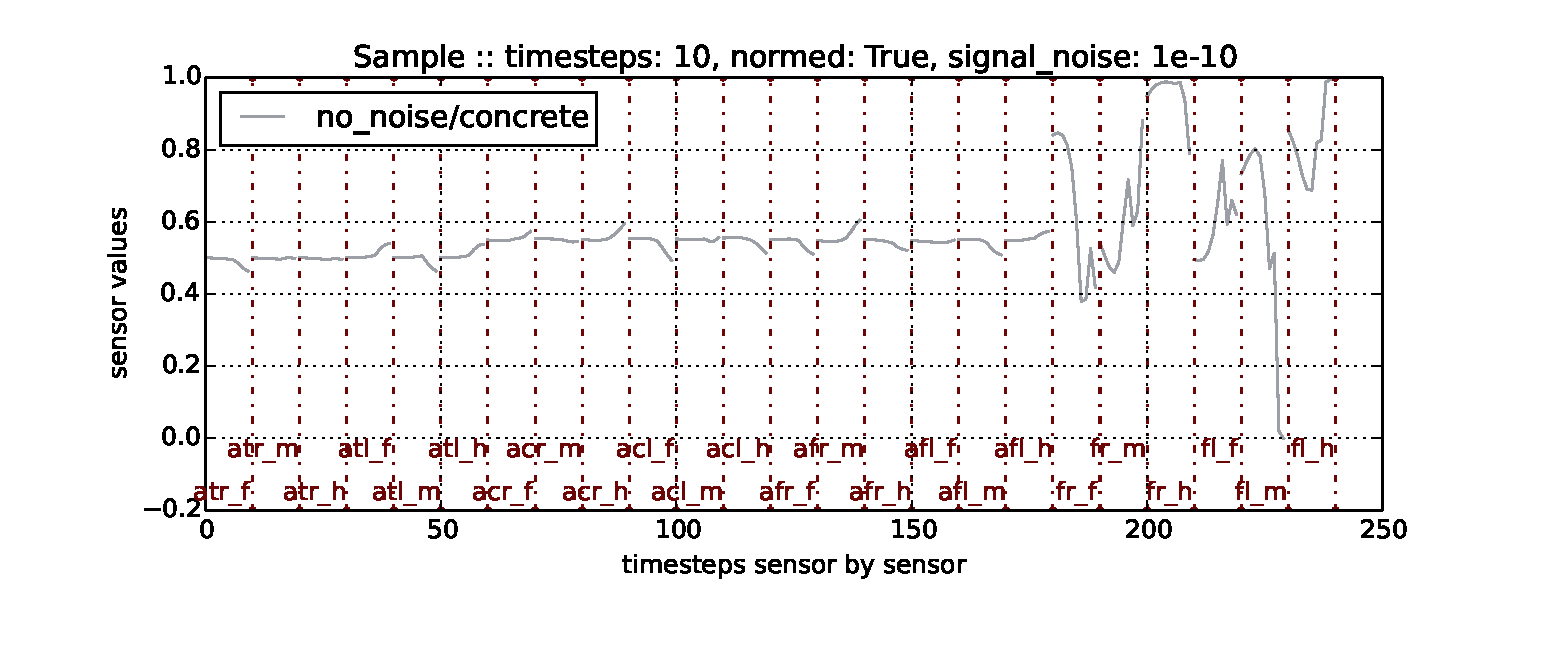
\includegraphics[width=1.0\textwidth]{sample_example_normed.eps}
  \caption{Example of feature vector - normed.}
  \label{fig:sample_example_normed}
\end{figure}

\subsection{Signal Noise} \label{ssec:signal_noise}
In \cref{ssec:terrain_noise} a few general reasons for noising simulation data are disscused. In that case an additive Gaussian noise is used to make the terrains definitions (from \cref{tab:terrains_parameters}) more complex.

For similar reasons also a signal noise is added to the data. In reality the mechanical sensors might shake, be influenced by environmental conditions or simply may not work as well as expected, while data coming from the simulated sensors are always deterministic.

\section{Datasets}
transformation into datasets, splitting into training-validation-testing sets

\section{Training and Classification}

Neural net training with several parameters and comparison with training with scikit-neuralnetwork library

2-3 pages

\subsection{Scikit-neuralnetwork library}
brief description of the library and its usage 1/2 pages

1 page